\section[简并态微扰论]{简并态微扰论} \label{sec:06.02} % 
% \makebox[5em][s]{} % 短题目拉间距

非简并态微扰论的特点是,受微扰作用后,原来的($\hat{H}_{0}$的)能级与本征函数都只发生微小的变化,$\varPsi_{n}^{(0)}\rightarrow\varPsi_{n}$,$E_{n}^{(0)}\rightarrow E_{n}$.简并态就不同,在微扰作用下,能级将发生分裂.

仍设$\hat{H}=\hat{H_{0}}+\hat{H}^{\prime}$,$\hat{H}^{\prime}$是微扰,设$\hat{H_{0}}$的某个能级$E_{n}^{(0)}$是$f$重简并的,有$f$个互相独立并且正交归一化的本征函数,
\begin{empheq}{equation}\label{eq62.1}
	\hat{H_{0}}\varPsi_{n\alpha}^{(0)}=E_{n}^{(0)}\varPsi_{n\alpha}^{(0)},\quad \alpha=1,2,\cdots,f
\end{empheq}
微扰$H^{\prime}$的存在一般地将引起这些本征态之间的耦合,因此,求解总能量的本征方程
\begin{empheq}{equation}\label{eq62.2}
	\hat{H}\varPsi_{n}=(\hat{H_{0}}+\hat{H}^{\prime})\varPsi_{n}=E_{n}\varPsi_{n}
\end{empheq}
时,$\varPsi_{n}$的零级近似一般应该是$\varPsi_{n\alpha}^{(0)}$的线性叠加,
\begin{empheq}{equation}\label{eq62.3}
	\varPsi_{n}^{(0)}=\sum_{\alpha}C_{\alpha}^{(0)}\varPsi_{n\alpha}^{(0)}
\end{empheq}
$\varPsi_{n}$的各级微扰修正仍记为$\varPsi^{(1)}$,$\varPsi^{(2)}$,$\cdots$,能级$E_{n}$的各级修正仍记为$E^{(1)}$,$E^{(2)}$,$\cdots$,即设
\begin{empheq}{align}
	\varPsi_{n}=\varPsi_{n}^{(0)}+\varPsi^{(1)}+\varPsi^{(2)}+\cdots	\label{eq62.4}\\
	E_{n}=E_{n}^{(0)}+E^{(1)}+E^{(2)}+\cdots		\label{eq62.5}
\end{empheq}
和上节一样,仍规定$\varPsi^{(1)}$,$\varPsi^{(2)}$,$\cdots$等不含$\varPsi_{n\alpha}^{(0)}$项,因此它们均和$\varPsi_{n\alpha}^{(0)}$正交,即
\begin{empheq}{align}\label{eq62.6}
	\langle \varPsi_{n\alpha}^{(0)}|\varPsi^{(1)} \rangle =0,\quad \langle \varPsi_{n\alpha}^{(0)}|\varPsi^{(2)} \rangle=0,\cdots
\end{empheq}
$\hat{H_{0}}$的其他($E_{n}^{(0)}$以外的)能级仍记为$E_{k}^{(0)}$,本征函数(不论是否简并)记为$\varPsi_{k}^{(0)}$
\begin{empheq}{equation}\label{eq62.7}
	\varPsi^{(1)}=\sum_{k}^{\prime}C_{k}^{(1)}\varPsi_{k}^{(0)}
\end{empheq}
将\eqref{eq62.4}、\eqref{eq62.5}式代入能量本征方程\eqref{eq62.2},并将各项按量级分开,形式上仍得到\eqref{eq61.9}列式,但必须牢记,现在由\eqref{eq61.3}式表示,它是$f$个简并态的线性叠加.

为了求出\eqref{eq62.3}式中各系数$C_{\alpha}^{(0)}$,以及能级的一级修正$E^{(1)}$,以各$\varPsi_{n\alpha}^{(0)*}(\alpha=1,2,\cdots,f)$轮流地左乘\eqref{eq61.9b}式,并对全空间积分,考虑到正交条件\eqref{eq62.6}式,即可得到下列关于$C_{\alpha}^{(0)}$的方程组:
\eqllong
\begin{empheq}{equation}\label{eq62.8}
	\begin{aligned}
		\begin{dcases}
			(H_{11}^{\prime}-E^{(1)})C_{1}^{(0)}+H_{12}^{\prime}C_{2}^{(0)}+\cdots+H_{1f}^{\prime}C_{f}^{(0)}=0	\\
			H_{21}^{\prime}C_{1}^{(0)}+(H_{22}^{\prime}-E^{(1)})C_{2}^{(0)}+\cdots+H_{2f}^{\prime}C_{f}^{(0)}=0	\\
			\qquad\qquad\qquad\quad\cdots\cdots\cdots\cdots	\\
			H_{f1}^{\prime}C_{1}^{(0)}+H_{f2}^{\prime}C_{2}^{(0)}+\cdots+(H_{ff}^{\prime}-E^{(1)})C_{f}^{(0)}=0
		\end{dcases}
	\end{aligned}
\end{empheq}\eqnormal
其中
\begin{empheq}{align}\label{eq62.9}
	H_{\alpha\beta}^{\prime}&\equiv H_{n\alpha,n\beta}=\int\varPsi_{n\alpha}^{(0)*}\hat{H}^{\prime}\varPsi_{n\beta}^{(0)}d\tau	\nonumber\\
	&=\langle \varPsi_{n\alpha}^{(0)}|\hat{H}^{\prime}|\varPsi_{n\beta}^{(0)} \rangle 
\end{empheq}
注意,\eqref{eq62.8}式中只出现$\{\varPsi_{n\alpha},\alpha=1,2,\cdots,f\}$子态矢空间中$\hat{H}^{\prime}$的矩阵元.实际上,\eqref{eq62.8}式相当于这子空间中微扰$\hat{H}^{\prime}$的本征方程,即
\eqlong
\begin{empheq}{equation*}\label{eq62.8'}
\begin{bmatrix}
	H_{11}^{\prime} & H_{12}^{\prime} & \cdots & H_{1f}^{\prime}	\\
	H_{21}^{\prime} & H_{22}^{\prime} & \cdots & H_{2f}^{\prime}	\\
	     \vdots     &      \vdots     &        & \vdots				\\
	H_{f1}^{\prime} & H_{f2}^{\prime} & \cdots & H_{ff}^{\prime}	\\
\end{bmatrix}\begin{bmatrix}
	C_{1}^{(0)}	\\	C_{2}^{(0)}	\\	\vdots	\\	C_{f}^{(0)}	\\
\end{bmatrix}=E^{(1)}\begin{bmatrix}
	C_{1}^{(0)}	\\	C_{2}^{(0)}	\\	\vdots	\\	C_{f}^{(0)}	\\
\end{bmatrix}
\end{empheq}
按照线性代数理论,\eqref{eq62.8}式存在非平庸解($C_{\alpha}^{(0)}$不全为0)的充要条件是
\begin{empheq}{equation}\label{eq62.10}
\begin{vmatrix}
	H_{11}^{\prime}-E^{(1)}	& H_{12}^{\prime} & \cdots & H_{1f}^{\prime}	\\
	H_{21}^{\prime}	& H_{22}^{\prime}--E^{(1)} & \cdots & H_{2f}^{\prime}	\\
	     \vdots     &      \vdots     &        & \vdots				\\
	H_{f1}^{\prime}	& H_{f2}^{\prime} & \cdots & H_{ff}^{\prime}-E^{(1)}	\\
\end{vmatrix}=0
\end{empheq}\eqnormal
亦即在$|\varPsi_{n\alpha}^{(0)}|$子空间中
\eqshort
\begin{empheq}{equation*}\label{eq62.10'}
	\det|H^{\prime}-E^{(1)}|=0
\end{empheq}
\eqref{eq62.10}式是$E^{(1)}$的$f$次代数方程,原则上可以求得$f$个$E^{(1)}$值,亦即原来的简并能级$E_{n}^{(0)}$在微扰论一级近似下已经分裂成为一组互相接近的能级.如\eqref{eq62.10}式的$f$个根互不重合,这表明在一级近似下能级$E_{n}^{(0)}$的简并化已经全部消除;如\eqref{eq62.10}式有重根,则表示简并化只是部分地消除.将由\eqref{eq62.10}式解出的每一个$E^{(1)}$值代回\eqref{eq62.8}式,求出$C_{\alpha}^{(0)}(\alpha=1,2,\cdots,f)$,并将其归一化,再代入\eqref{eq62.3}式,就得到和这个$E^{(1)}$相应的零级近似波函数.

有一种重要情况值得特别指出.如上述$f$个简并态中有一个特殊的$\varPsi_{n\beta}^{(0)}$,它与其他$\varPsi_{n\alpha}^{(0)}$构成的微扰矩阵元全部等于零,即$H_{\alpha\beta}^{\prime}=0$,则\eqref{eq62.8}式中唯一出现$C_{\beta}^{(0)}$的式子是
\begin{empheq}{equation*}
	(H_{\beta\beta}^{\prime}-E^{(1)})C_{\beta}^{(0)}=0
\end{empheq}\eqnormal
这时\eqref{eq62.8}式显然有特解
\begin{empheq}{equation*}
	E^{(1)}=H_{\beta\beta}^{\prime},\quad C_{\beta}^{(0)}=1,\quad C_{\alpha}^{(0)}=0(\alpha\neq\beta)
\end{empheq}
亦即$\varPsi_{n\beta}^{(0)}$单独构成正确的零级波函数,$E^{(1)}$等于微扰$H^{\prime}$的平均值.处理简并态微扰论问题,首先应该找出(如果有的话)这种特殊状态,问题就可得到简化.

波函数的一级修正$\varPsi^{(1)}$和能级的二级修正$E^{(2)}$也可以仿照$\S$\ref{sec:06.01}的程序而求出.$E^{(2)}$仍由\eqref{eq61.11}式表示,即
\eqlong
\begin{empheq}{equation}\label{eq62.11}
	E^{(2)}=\int\varPsi_{n}^{(0)*}\hat{H}^{\prime}\varPsi^{(1)}d\tau=\langle \varPsi_{n}^{(0)}|\hat{H}^{\prime}|\varPsi^{(1)} \rangle 
\end{empheq}\eqnormal
$\varPsi^{(1)}$由\eqref{eq62.7}式表示,$C_{k}^{1}$的公式仍可仿照$\S$\ref{sec:06.01}的程序求得,
\eqindent{1}
\begin{empheq}{equation}\label{eq62.12}
	C_{k}^{(1)}=\frac{\langle \varPsi_{k}^{(0)}|\hat{H}^{\prime}|\varPsi_{n}^{(0)} \rangle }{E_{n}^{(0)}-E_{k}^{(0)}}=\frac{1}{E_{n}^{(0)}-E_{k}^{(0)}}\sum_{\alpha}C_{\alpha}^{(0)}\langle \varPsi_{k}^{(0)}|\hat{H}^{\prime}|\varPsi_{n\alpha}^{(0)} \rangle 
\end{empheq}\eqnormal	\eqlong
\begin{empheq}{align}\label{eq62.13}
	\varPsi^{(1)}&=\sum_{n}^{\prime}\frac{1}{E_{n}^{(0)}-E_{k}^{(0)}}\langle \varPsi_{k}^{(0)}|\hat{H}^{\prime}|\varPsi_{n}^{(0)} \rangle\varPsi_{k}^{(0)}	\nonumber\\
	&=\sum_{k}^{\prime}\frac{\varPsi_{k}^{(0)}}{E_{n}^{(0)}-E_{k}^{(0)}}\sum_{\alpha}C_{\alpha}^{(0)}\langle \varPsi_{k}^{(0)}|\hat{H}^{\prime}|\varPsi_{n\alpha}^{(0)} \rangle
\end{empheq}
矩阵元$\langle \varPsi_{n}^{(0)}|\hat{H}^{\prime}|\varPsi_{n\alpha}^{(0)}\rangle$表示$\varPsi_{n\alpha}^{(0)}$态与$\varPsi_{k}^{(0)}$态由于$\hat{H}^{\prime}$的作用而产生耦合,因此(一级近似)波函数中出现$\varPsi_{k}^{(0)}$项.

将\eqref{eq62.13}式代入\eqref{eq62.11}式,即可得出$E^{(2)}$的具体表示式:
\begin{empheq}{align}\label{eq62.14}
	E^{(2)}&=\sum_{n}^{\prime}\frac{1}{E_{n}^{(0)}-E_{k}^{(0)}}\langle \varPsi_{n}^{(0)}|\hat{H}^{\prime}|\varPsi_{k}^{(0)} \rangle\langle \varPsi_{k}^{(0)}|\hat{H}^{\prime}|\varPsi_{n}^{(0)} \rangle	\\
	&=\sum_{k}^{\prime}\frac{1}{E_{n}^{(0)}-E_{k}^{(0)}}\sum_{\alpha,\beta}C_{\alpha}^{(0)}C_{\beta}^{(0)*}H_{n\beta,k}H_{k,n\alpha}	\nonumber	%\tag{$6.2.14^{\prime}$}
\end{empheq}
上式表明,能级的二级微扰修正$E^{(2)}$来源于微扰$H^{\prime}$引起的$\varPsi_{n}^{(0)}$态与其他各能级态$\varPsi_{k}^{(0)}$的耦合,矩阵元$\langle \varPsi_{k}^{(0)}|\hat{H}^{\prime}|\varPsi_{n}^{(0)}\rangle$就代表这种耦合.由于$\varPsi_{n}^{(0)}$系由$f$个简并态$\varPsi_{n\alpha}^{(0)},\varPsi_{n\beta}^{(0)},\cdots$组成,因此具体表现为下列形式的耦合:
\begin{empheq}{equation*}
	\varPsi_{n\alpha}^{(0)}\stackrel{H^{\prime}}{——}\varPsi_{k}^{(0)}\stackrel{H^{\prime}}{——}\varPsi_{n\beta},\quad \alpha,\beta=1,2,\cdots,f
\end{empheq}\eqnormal
而对于非简并能级,与$E_{n}^{(0)}$相应的状态只有一个$\varPsi_{n}^{(0)}$,二级能量修正$E_{n}^{(2)}$相应于耦合$\varPsi_{n}^{(0)}-\varPsi_{k}^{(0)}-\varPsi_{n}^{(0)}$,$E_{k}^{(0)}\neq E_{n}^{(0)}$.

处理简并态微扰论问题,核心目标是弄清楚能级的分裂情况.如在一级近似下,能级已经分裂,简并已经消除,[与此相应,各个零级波函数$\varPsi_{n}^{(0)}$也可经由\eqref{eq62.8}式确定下来]一般就不必再计算能级的二级修正和波函数的一级修正.[如有必要,可按\eqref{eq62.13}、\eqref{eq62.14}式计算.]如在能量一级近似下,简并并未完全消除,则对于仍然简并的那些能级,零级波函数实际上无法经由\eqref{eq62.8}式而确定下来,因此\eqref{eq62.13}、\eqref{eq62.14}式实际上无法使用.这种情况下,需要重新处理,$\varPsi_{n}^{(0)}$将与$E^{(2)}$(甚至$E^{(3)}$,$\cdots$)同时求出,亦即能级分裂发生在高级近似下.

\example 研究氢原子的第二个能级在外电场中引起的分裂,即史塔克效应.(计算能级的一级修正,不考虑电子自旋.)

\solution 以$E_{n}^{(0)}$和$\varPsi_{nlm}^{(0)}$表示孤立氢原子的能级和能量本征态($H_{0},\boldsymbol{L}^{2},L_{z}$的共同本征态).能级$E_{n}^{(0)}$的简并度是$n^{2}$,第二个能级$E_{2}U(0)$共有4个本征态,$nlm$值为
\begin{empheq}{equation*}
	nlm=200,210,211,21-1
\end{empheq}
$\varPsi_{nlm}^{(0)}$可以表示成(参看$\S$\ref{sec:05.01},$\S$\ref{sec:05.04})
\begin{empheq}{equation*}
	\varPsi_{nlm}^{(0)}=R_{nl}(r)Y_{lm}(\theta,\varphi)
\end{empheq}
与本题有关的径向波函数只有2种,$R_{21}$及$R_{20}$,$Y_{lm}$则有4种,它们是
\begin{empheq}{align*}
	Y_{00}&=\sqrt{\frac{1}{4\pi}}	\\
	Y_{10}&=\sqrt{\frac{3}{4\pi}}\cos\theta=\sqrt{\frac{3}{4\pi}}\frac{z}{r}	\\
	Y_{11}&=-\sqrt{\frac{3}{8\pi}}\sin\theta e^{i\varphi}=-\sqrt{\frac{3}{8\pi}}\frac{x+iy}{r}	\\
	Y_{1-1}&=\frac{3}{8\pi}\sin\theta e^{-i\varphi}
\end{empheq}

将氢原子置于电场$\mathscr{E}$中,以电场方向作为$z$轴,则电场对电子的作用势为
\begin{empheq}{equation}\label{eq62.15}
	H^{\prime}=e\mathscr{E}\cdot\boldsymbol{r}=e\mathscr{E}z=e\mathscr{E}r\cos\theta
\end{empheq}
如电场强度$\mathscr{E}$不超过$10^{6}$\si{V/cm},则$H^{\prime}$的数量级为
\begin{empheq}{equation*}
	H^{\prime}<(10^{6}\si{eV/cm})(10^{-8}\si{cm})=10^{-2}\si{eV}
\end{empheq}
而电子能级间距为几个电子伏,所以$H^{\prime}$可以当作微扰.

由于$\hat{H}^{\prime}$和$\hat{L_{z}}$对易,$\hat{H}^{\prime}$作用于$\varPsi_{nlm}^{(0)}$的结果,$\hat{L_{z}}$的取值$(m\hbar)$不变.由于$\hat{H}^{\prime}$是奇宇称,所以在任何$\varPsi_{nlm}^{(0)}$态下$H^{\prime}$的平均值为0.这样一来,在上述4个简并态组成的子空间中,凡和(211)及(21-1)态有关的$H^{\prime}$矩阵元全部为0,也就是说,在波函数的零级近似中,$H^{\prime}$的作用并不能使(211)、(21-1)态与其他简并态发生耦合,它们就是正确的零级波函数,而且不受$H^{\prime}$影响,能级不发生变化(一级近似).

在$n=2$的上述态矢空间中,仅有的不等于零的$H^{\prime}$矩阵元是
\begin{empheq}{align*}
	H_{200,210}^{\prime}&=H_{210,200}^{\prime}=e\mathscr{E}\int z\varPsi_{200}\varPsi_{210}d\tau	\\
	&=\frac{e\mathscr{E}}{\sqrt{3}}\int_{0}^{\infty}r^{3}R_{20}R_{21}dr
\end{empheq}
径向波函数的具体函数形式见\eqref{eq54.27}、\eqref{eq54.28}式,经过简单计算,得到
\begin{empheq}{equation}\label{eq62.16}
	H_{200,210}^{\prime}=H_{210,200}^{\prime}=-3e\mathscr{E}a_{0}
\end{empheq}
$a_{0}=\frac{\hbar^{2}}{\mu\e^{2}}$是玻尔半径.读者如能注意到$Y_{lm}$和$H^{\prime}$在直角坐标系中的对称性(奇偶性),当能对上述关于$H^{\prime}$矩阵元的讨论加深印象.

至此,初步结论是,在外电场作用下,4个简并态中(211)态和(21-1)态并不与其他态耦合,能级仍保持原来的值.(200)态和(210)态则产生耦合,这将导致能级分裂.将简并态微扰论用于这两个简并态,令
\begin{empheq}{equation}\label{eq62.17}
	\varPsi_{n}^{(0)}=C_{1}^{(0)}\varPsi_{200}^{(0)}+C_{2}^{(0)}\varPsi_{210}^{(0)}
\end{empheq}
\eqref{eq62.8}式具体表现为
\begin{empheq}{equation}\label{eq62.18}
	{}\begin{dcases}
		E^{(1)}C_{1}^{(0)}+3e\mathscr{E}a_{0}C_{2}^{(0)}=0	\\
		3e\mathscr{E}a_{0}C_{1}^{(0)}+E^{(1)}C_{2}^{(0)}
	  \end{dcases}
\end{empheq}
\eqref{eq62.10}式表现为
\begin{empheq}{equation}\label{eq62.19}
	(E^{(1)})^{2}-(3e\mathscr{E}a_{0})^{2}=0
\end{empheq}
解为
\eqshort
\begin{empheq}{equation*}
	E^{(1)}=\pm3e\mathscr{E}a_{0}
\end{empheq}\eqnormal
此即能级$E_{2}^{(0)}$的一级微扰分裂(一级史塔克效应).再由\eqref{eq62.18}式可求出$C_{1}^{(0)}$,$C_{2}^{(0)}$,结果为
\eqllong
\begin{empheq}{equation}\label{eq62.20}
	\begin{aligned}
		E^{(1)}&=3e\mathscr{E}a_{0},\quad C_{1}^{(0)}=-C_{2}^{(0)},\quad 
		\varPsi^{(0)}=\frac{1}{\sqrt{2}}(\varPsi_{200}^{(0)}-\varPsi_{210}^{(0)})	\\
		E^{(1)}&=-3e\mathscr{E}a_{0},\quad C_{1}^{(0)}=C_{2}^{(0)},\quad 
		\varPsi^{(0)}=\frac{1}{\sqrt{2}}(\varPsi_{200}^{(0)}+\varPsi_{210}^{(0)})
	\end{aligned}
\end{empheq}\eqnormal
能级分裂如图\ref{fig.6-1}所示.

\begin{figure}[!h]
	\centering
	\small
	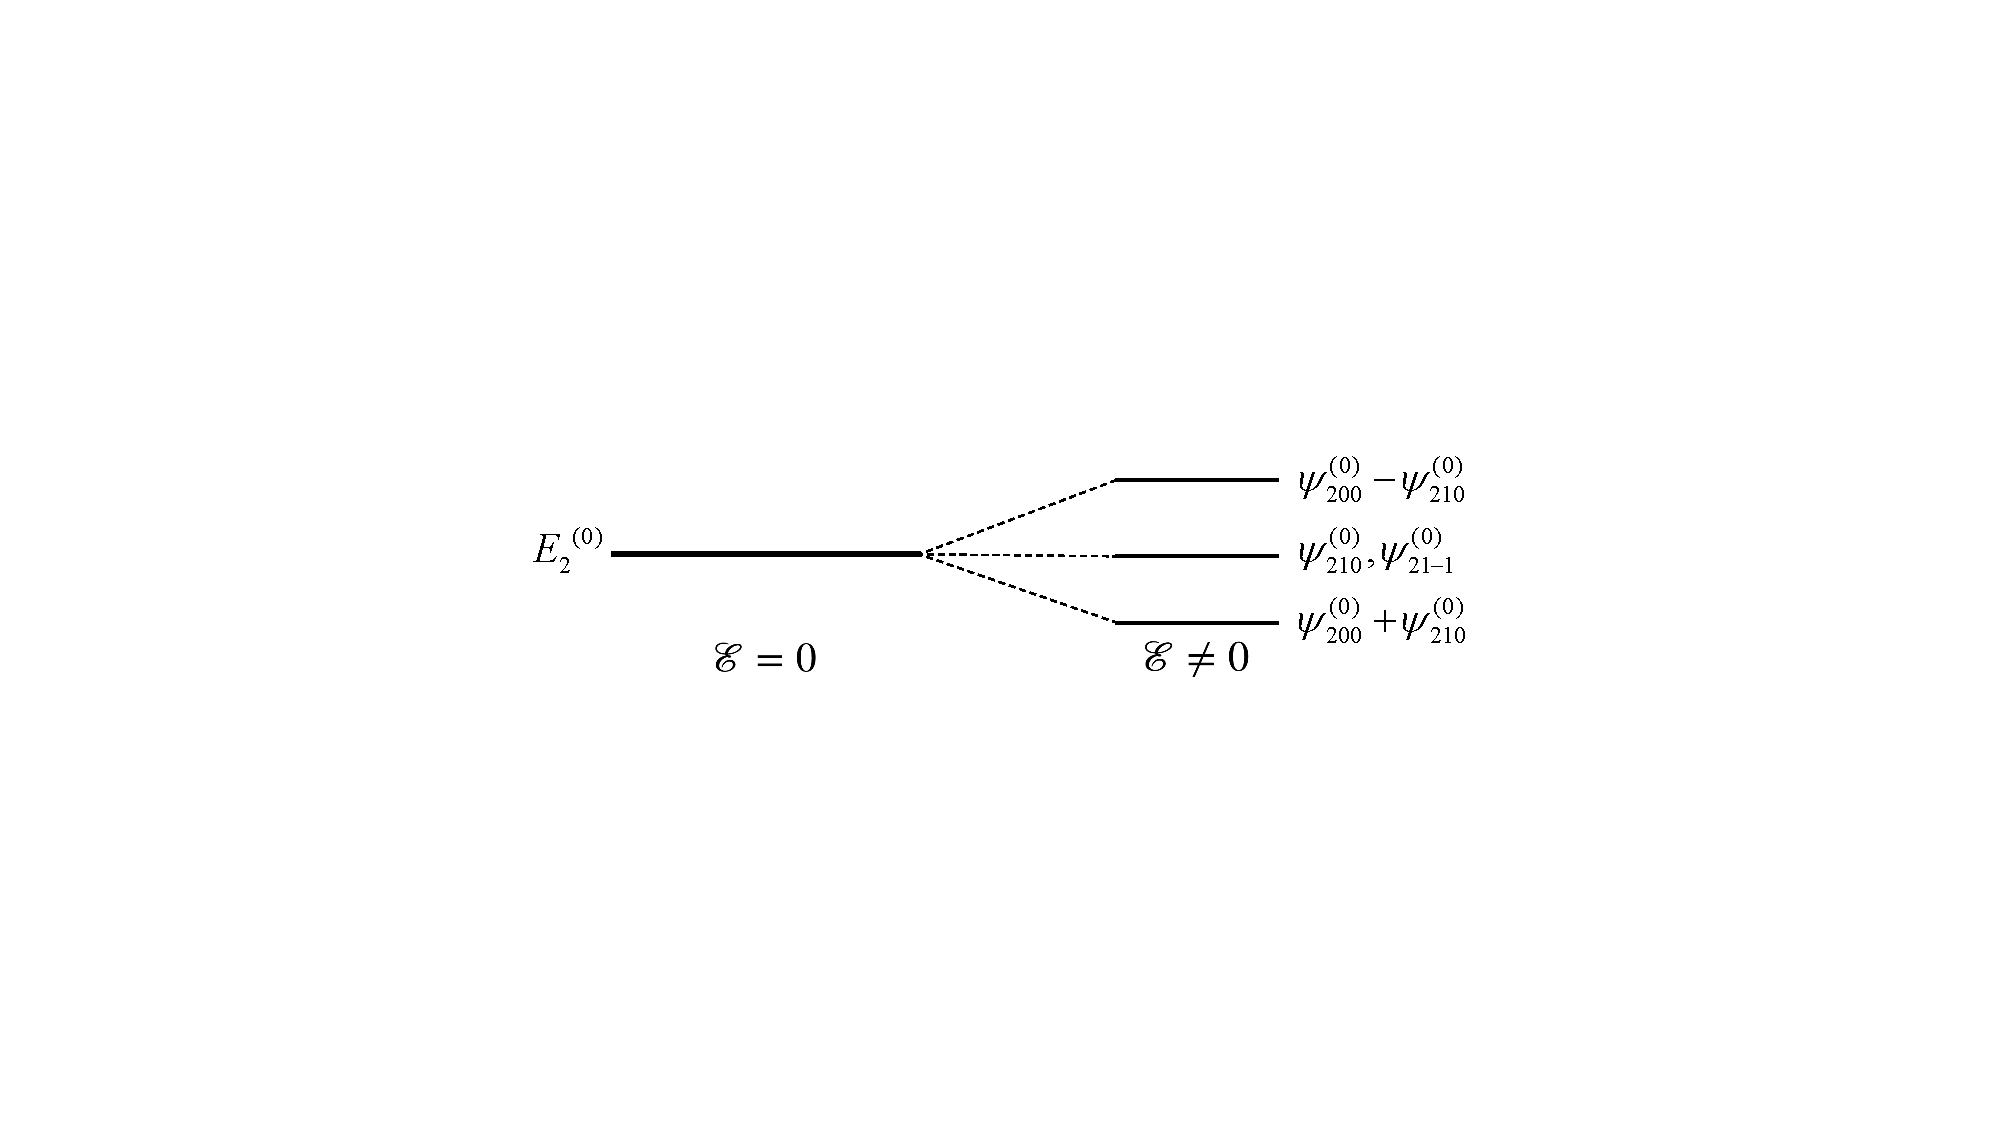
\includegraphics[width=6cm,clip]{QM file/figure/6-1}
	\caption{}\label{fig.6-1}
\end{figure}

值得注意的是原子的物理性质在外电场作用下发生的变化,氢原子的电偶极矩算符为
\eqshort
\begin{empheq}{equation}\label{eq62.21}
	\boldsymbol{D}=-e\boldsymbol{r}
\end{empheq}\eqnormal
未加电场时,原子的定态$\varPsi_{nlm}^{(0)}$均有或奇或偶的宇称,而$\boldsymbol{D}$为奇宇称,因此$\boldsymbol{D}$的平均值为0.在电场$\mathscr{E}$作用下,分裂出两个新的能级$E_{2}^{(0)}\pm3e\mathscr{E}a_{0}$,相应的波函数由\eqref{eq62.20}式表示,它们都是$\varPsi_{200}^{(0)}$和$\varPsi_{210}^{(0)}$的耦合态,已经没有宇称性,平均电矩也不为零,计算结果是
\eqlong
\begin{empheq}{align*}
	\varPsi^{(0)}&=\frac{1}{\sqrt{2}}(\varPsi_{200}^{(0)}-\varPsi_{210}^{(0)}),\quad \overline{D_{x}}=\overline{D_{y}}=0,\quad \overline{D_{z}}=-3ea_{0}	\\
	\varPsi^{(0)}&=\frac{1}{\sqrt{2}}(\varPsi_{200}^{(0)}+\varPsi_{210}^{(0)}),\quad \overline{D_{x}}=\overline{D_{y}}=0,\quad \overline{D_{z}}=3ea_{0}
\end{empheq}\eqnormal
正是耦合态的这个固有电矩在外电场中获得的势能
\begin{empheq}{equation*}
	E^{(1)}=0\langle \mathscr{E}\cdot\boldsymbol{D} \rangle=-\mathscr{E}\overline{D_{z}}=\pm3e\mathscr{E}a_{0}
\end{empheq}
造成了能级分裂.
